\chapter{Auswahl \& Konzept}
\section{Endergebnis und Empfehlung}
Nach Abschluss des Evaluierungsprozesses ist das Projektteam an diesem Punkt in der Lage eine Empfehlung an das Unternehmen Kapsch auszusprechen. In diesem Teil wird nun erläutert, welches evaluierte Konzept mit den Anforderungen des Auftraggebers übereinstimmt und wodurch dies zu Stande gekommen ist. Nachdem die Linuxmanipulation aus Garantietechnischen Gründen bereits als ausgeschieden gilt, befasst sich der folgende Abschnitt nur mehr mit den Konzepten MDM\footnote{Mobile Device Management}, MDM + Container und Samsung Knox.
\section{Evaluierung}
Um feststellen zu können welche der 3 Lösungen am besten die Anforderungen des Auftraggebers erfüllen kann, hat das Projektteam eine Nutzwertanalyse erstellt, mit derer Hilfe das Projektteam die Funktionen der Systeme direkt miteinander vergleichen konnten.
\subsection{Nutzwertanalyse}
Die Tabelle auf der folgenden Seite zeigt den Vergleich zwischen Mobile Device Management, Mobile Device Management + Container und Samsung Knox in form einer Nutzwertanalyse.

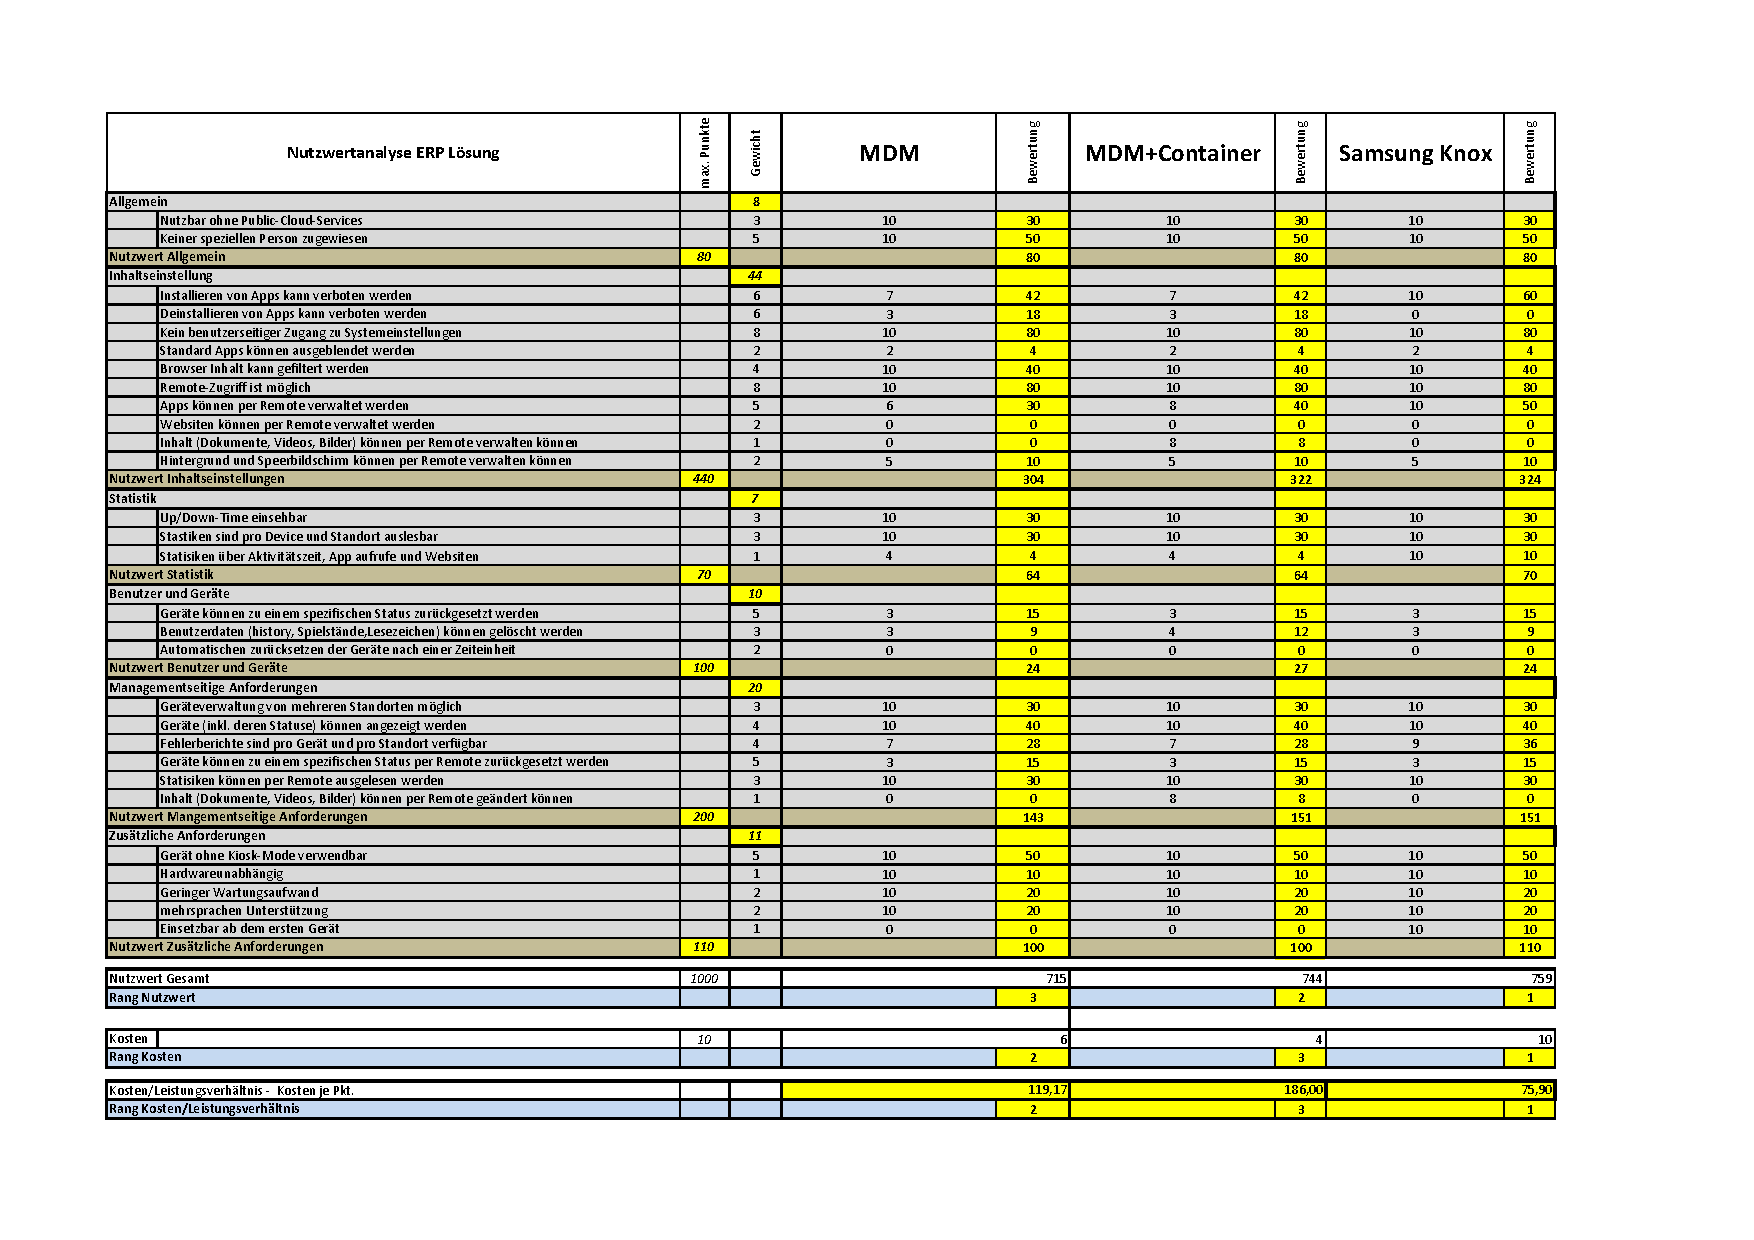
\includepdf[landscape]{nutzwertanalyse}

\section{Auswertung der Evaluierung}
Um eine aussagekräftiges Ergebnis zu erhalten, wurden die Anforderungen des Gesamtsystems in verschiedene Unterpunkte unterteilt, welche auf ihre Funktionstüchtigkeit hin untersucht wurden. \par
Die Lösungen wurden dann je nach Erfüllungsgrad der einzelnen Punkte bewertet, was eine objektive Vergleichbarkeit schaffen sollte.
\subsection{Allgemein}
Da alle drei Systeme sowohl ohne pulic-cloud-service nutzbar waren als auch keiner speziellen Person zugewiesen werden müssen, haben die alle drei Lösungen volle Punkte erreich und sind somit was diesen Punkt angeht gleich auf.
\subsection{Inhaltseinstellungen}
In diesem Bereich hat sich herausgestellt ist Samsung Knox kapp aber doch noch vor der MDM+Container Lösung das am besten geeignete System. Denn auch wenn es mit MDM+Containern möglich ist, die Deinstallation von betriebsinternen Apps zu verbieten und man auch Inhalte der Geräte wie zum Beispiel Bilder, Dokumente, etc per remote verwalten kann, ist Samsung die hier die bessere Alternative, da es eine bei weitem bessere Verwaltung von Apps per Remote bietet. \par
Eine Anforderung die jedoch keines der drei Systeme erfüllen konnte war das Verwalten von Websiten per remote.
\subsection{Statistik}
Auch den Unterpunkt Statistiken kann Samsung Knox wieder für sich entscheiden. Diesmal jedoch mit einem Größeren Vorsprung. Zurückzuführen ist das darauf, dass Samsung Knox die Möglichkeit bietet, sich jede beliebige Statistik die man für sein Unternehmen haben will, einfach mittels SQL Code selbst zu erzeugen(siehe Punkt 8.3.1 Statistiken).
\subsection{Benutzer und Geräte}
In diesem Bereich kann die MDM+Container Lösung punkten. Denn im Gegensatz zu den anderen zwei Systemen, kann man mit dieser Lösung am Gerät gespeicherte Lesezeichen löschen. \par
Auch bei diesem Unterpunkt gibt es wieder eine Anforderung die mit keinem unserer getesteten Systeme umsetzbar war. Und zwar war es nicht möglich die Geräte so zu konfigurieren, dass sie sich nach einer gewissen Zeit von alleine auf einen definierten Stand zurücksetzen.
\subsection{Managementseitige Anforderungen}
Bei der Erfüllung der Managementseitigen Anforderungen sind Samsung Knox und die MDM+Container-Lösung gleich auf. Denn den Vorsprung den Knox gewinnt durch besseres Handling der Fehlerberichte, kann die MDM+Container-Lösung dadurch wegmachen, das sie im Gegensatz zu Samsung Knox eine Möglichkeit bietet, Geräteinhalt per remote zu ändern.
\subsection{Zusätzliche Anforderungen}
Da Samsung Knox das einzige System ist, welches bereits ab dem ersten Gerät einsetzbar ist und sonst alle Punkte von allen Systemen erfüllt werden ist auch hier Knox der klare Sieger.

\section{Empfehlung}
Nach eingehender Analyse ist das Projektteam zu dem Schluss gekommen, dass für die geplanten Projekte der Firma die Betriebsplattform Samsung Knox am ehesten geeignet ist. Es implementiert die meisten der benötigten Features, aber lässt dennoch einige fundamentale Punkte aus. Deshalb ist es hier für das Projektteam auch nicht möglich eine hundert prozentige Empfehlung zu geben. Den Informationen der Dokumentation von Samsung Knox zur Folge werden einige benötigte Features in kommenden Versionen eingebaut. Allerdings ist nicht absehbar ob und wann diese erscheinen. Für die beiden anderen Systeme kann deshalb keine Empfehlung ausgesprochen werden, weil sie weniger und besonders im Einsatz mit Nicht-Samsung-Geräten signifikant weniger Funktionen bieten.

